At the time of writing there are no publicly available implementations of HQC specifically targeting microcontrollers.
In this section we describe our implementation of HQC targeting ARM Cortex-M4 microcontrollers, showing the implementative
details for various multiplication algorithms; moreover, we show the first fully masked implementation of HQC, as a countermeasure
against power side-channel attacks.

\section{Polynomial multiplication}
From a computational standpoint, the most expensive operations in HQC are by far the polynomial multiplications: for this reason,
in order to achieve good performance, it is crucial to pick the best multiplication algorithm for the target architecture.

    The polynomials $v \in \mathcal{R}$ can be represented in two possible forms:
    \begin{itemize}
        \item sparse, as a vector of size $\omega$ coefficients, $\omega = \texttt{wt}(v)$, where each entry corresponds to the degree of a non-zero coefficient.
        \item dense, as a vector of size $\lceil \frac{n}{\texttt{ws}} \rceil$, where \texttt{ws} is the word size of the target architecture.
    \end{itemize}
    With the aforementioned parameters, the objects on which HQC operates require the amounts of memory summarized in Table~\ref{tab:memory}.
    \begin{table}[ht]\small
        \centering
        \caption{Memory consumption (in bytes)}
        % as wide as the page
        \begin{tabular}{c|c|c|c|c|c|c}
            Instance & Message & Secret Key & Public Key  & Ciphertext & Dense Poly & Sparse Poly \\
            \hline 
            \texttt{hqc-128} & 16 & 2289 & 2249 & 4481 & 2209 & 300\\
            \hline
            \texttt{hqc-192} & 24 & 4562 & 4522 & 9026 & 4482 & 456\\
            \hline
            \texttt{hqc-256} & 32 & 7285 & 7245 & 14469 & 7205 & 596\\
        \end{tabular}
        \label{tab:memory}
    \end{table}

Note that the secret key size refers to the memory required to store a $\textit{processable}$ version of if; the
secret key can also be stored as a 40B seed, which is then used to generate the actual key material.

Due to its large memory footprint and the limited resources of the target platform, we will consider only the \texttt{hqc-128} instance.


	% descrivere la moltiplicazione shift & add semplice
	\subsection{Shift and Add}\label{subsec:shift_add}
		In the third round reference implementation of HQC, the polynomial multiplication is implemented using a variant of the schoolbook
		\textit{shift and add} method, recalling that the multiplication in $\mathcal{R}$ of a polynomial by a monomial of degree $i$ 
		can be implemented as a circular shift to the left (\clshift) 	of $i$ positions. Given $a(x)$ in sparse form and $b(x)$ in dense form, the algorithms multiplies $b(x)$ by $x^w$, 
		for all $w$s, where $w$ is a non-zero coefficient of $a(x)$, and then adds the results together:

		\begin{algorithm2e}[H]
			\caption{Sparse polynomial multiplication}
			\KwIn{$a(x) \in \mathcal{R}_\omega$ in sparse form, $b(x) \in \mathcal{R}$ in dense form}
			\KwOut{$c(x) = a(x) \cdot b(x) \in \mathcal{R}$ in dense form}
			\For{$i \gets 0$ \KwTo \texttt{ts}}{
				$\texttt{table}[i] \gets b(x) \clshift i$\;
			}
			\For{$i \gets 0$ \KwTo $\texttt{wt}(a(x))$}{
				$w \gets a(x)[i]$\;
				$\texttt{dec} \gets w \mod \texttt{ts}$\;
				$\texttt{s} \gets \lfloor \frac{w}{\texttt{ts}} \rfloor$\;
				$\texttt{tmp} \gets x^\texttt{s}\cdot x^\texttt{ts}$\;
				$c(x) \gets c(x) + \texttt{table}[\texttt{dec}] \cdot \texttt{tmp}$\;
			}
			\KwRet $c(x) \mod (x^n+1)$\;
		\end{algorithm2e}
		The idea of this variant is to precompute the first \texttt{ts} shifts of $b(x)$ and store them in a table, where \texttt{ts} is set to 16;
		this allows to slightly improve the performance of the algorithm and to shuffle the memory accesses to \texttt{table}.\\
		Since $a$ is very sparse, this approach is extremely fast; however, the high speed achieved is counterbalanced by the
		non-constant time execution of the algorithm, which is a major drawback for the security of the implementation. 

	% descrivere la versione a tempo costante della mul shift & add 
	\subsection{Constant-time shift and add}\label{subsec:const_shift_add}
		Due to the high sparsity of one of the operands, we would like to exploit the fact that the algorithm is very fast to implement a constant-time version of it;
		such an algorithm is implemented in LEDAcrypt~\cite{DBLP:conf/cbc/BaldiBCPS19} and is based on \textit{shifts with conditional commitment}.\\

		\begin{algorithm2e}[H]
			\caption{Constant-time monomial multiplication}
			\KwIn{$a$ exponent of a monomial $x^a \in \mathds{Z}_2[x]$ with $0 \leqslant a < n$, \newline
					$b(x) \in \mathcal{R}$ in dense form}
			\KwOut{$c(x) = x^a \cdot b(x) \in \mathcal{R}$ in dense form}
			\KwData{$m = \lceil \log_2(a) \rceil$ number of bits needed to encode $a$ in binary, \newline
					\textit{i.e.} $a = (\beta_{m-1}, \cdots, \beta_0)_{\texttt{bin}}$}

			$c(x) \gets b(x) \clshift (a \mod \texttt{ws})$\;
			\For{$i \gets \log_2(\texttt{ws})$ \KwTo $(m-1)$} {
				$\texttt{tmp} \gets b(x) \clshift i$\;
				$c(x) \gets c(x) + \texttt{tmp}$\;
				$\texttt{cond} \gets (\beta_{i} == 1)$\;
				$\texttt{mask} \gets 0 - (\texttt{WORD})(\texttt{cond})$\;
				$c(x) \gets c(x) + ((c(x) \wedge \texttt{mask}) \vee (\texttt{tmp}(x) \wedge \texttt{mask}))$\;
			}
			\KwRet $c(x)$\;
		\end{algorithm2e}
		With this algorith we compute the $i$-th shift of $b(x)$ regardless of the value of $\beta_i$, but we sum it to the result only if
		$\beta_i = 1$ (the mask at line 6 contains either all zeros or all ones, '$\vee$' and '$\wedge$' correspond to the bitwise OR and AND respectively).
	% descrivere la moltiplicazione con trasformate

    \subsection{Frobenius Additive FFT}\label{subsec:fafft}
        The implementation of the Frobenius Additive FFT is based on the work of Chen \textit{et.al.}~\cite{DBLP:journals/tches/ChenCK21}; for the sake of clarity, 
        we highlight the core ideas of this implementation.
        
        As shown in Algorithm~\ref{alg:fafft}, the FAFFT multiplication is composed of four components (with the relative inverses): basis conversion, encoding, butterflies and
        pointwise multiplication.
        Our implementation targets a 32-bit platform, hence we pick $m=32$ for the ease of representation of the operands in memory; 
        recalling Equation~\ref{eq:frobenius_partition}, the optimal Frobenius partition for our parameters is $\Sigma = v_{27} + W_{11}$. 
        Since the degree of the operands is fixed, it is possible to optimize these algorithms by unrolling the recursive calls and precomputing the necessary tables.

    \subsubsection{Pointwise multiplication}
        To carry out the 2048 pointwise multiplications in $\mathds{F}_{2^{32}}$ the field elements are represented in a bitsliced format,
        where each element is stored in a memory word. Given  $a$ and $b$ elements in $\mathds{F}_{2^{32}}$, we can compute their product
        by splitting them as $a_0 + a_1\cdot x^{16}$ and $b_0 + b_1\cdot x^{16}$, and computing the product using the Karatsuba multiplication
        algorithm in $\mathds{F}_{2^{16}}$.

    \subsubsection{Basis conversion}
        In Algorithm~\ref{alg:basiscvt}, we show how to convert a polynomial from the canonical to the \emph{novelpoly} basis by recursively
        dividing the input by the vanishing polynomials $s_i(x)$. Since the division by the vanishing polynomial (of largest degree possible) always produces only $h_0(x)$ and $h_1(x)$, 
        we can unroll the recursive calls and transform the algorithm in a binary circuit with only \texttt{XOR} operations; moreover, we can remove all the operations on coefficients
        of the input polynomial that we know are zero.

        \begin{example}[Monomial to novelpoly basis conversion]
            Each step splits the input into quotient and remainder, so we can represent the whole algorithm as a tree, where a node's left child is the remainder and the right child is the quotient:
            by doing so, at the last step of the recursion we can read the leaves, from left to right, as the coefficients $g_0, g_1, \cdots$ of the polynomial in the novelpoly basis.

            Let us take $f(x) = x^6$ in monomial basis and apply the basis conversion algorithm to it. The greatest $i$ such that $2^{2^i} \leqslant \deg(f(x))$ is $i=2$, so at the various
            levels of the tree we will divide the inputs by $s_2(x)=x^4+x$ and $s_1(x)=x^2+x$:
            \begin{figure}[H]
                \caption{Expansion of the basis conversion algorithm for $f(x) = x^6$}
                \begin{center}
                    \begin{forest}
                        [$x^6$[$x^3$[0[0][0]][$x+1$[1][1]]][$x^2$[$x$[0][1]][1[1][0]]]]
                    \end{forest}
                \end{center}
                \label{fig:tree}
            \end{figure}
            hence the representation of $x^6$ in novelpoly basis is $X_2(x) + X_3(x) + X_5(x) + X_6(x)$.

            If we repeat the same procedure with all the required monomials (of degree less than 8 for this case) we can obtain the following circuit that maps coefficients of the 
            canonical basis $f_i$ to coefficients of the novelpoly basis $g_i$, where the dashed line marks the separation between the first two levels of the tree after the root:

            \begin{figure}[H]
    \caption{Basis conversion, $n < 8$}
    \begin{center}
        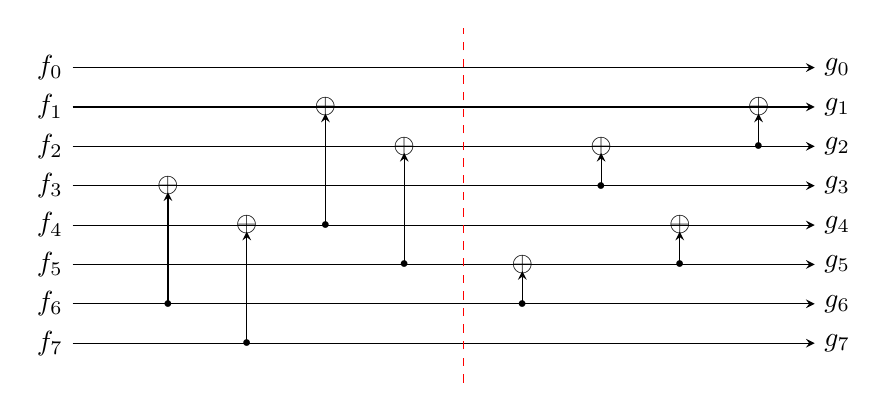
\begin{tikzpicture}[scale=0.5]
            \node (f0) at (0,7) {$f_0$};
            \node (f1) at (0,6) {$f_1$};
            \node (f2) at (0,5) {$f_2$};
            \node (f3) at (0,4) {$f_3$};
            \node (f4) at (0,3) {$f_4$};
            \node (f5) at (0,2) {$f_5$};
            \node (f6) at (0,1) {$f_6$};
            \node (f7) at (0,0) {$f_7$};
            \node (g0) at (20,7) {$g_0$};
            \node (g1) at (20,6) {$g_1$};
            \node (g2) at (20,5) {$g_2$};
            \node (g3) at (20,4) {$g_3$};
            \node (g4) at (20,3) {$g_4$};
            \node (g5) at (20,2) {$g_5$};
            \node (g6) at (20,1) {$g_6$};
            \node (g7) at (20,0) {$g_7$};

            \node (m1) at (3, 1)  {\tiny$\bullet$};
            \node (m2) at (5, 0)  {\tiny$\bullet$};
            \node (m3) at (7, 3)  {\tiny$\bullet$};
            \node (m4) at (9, 2)  {\tiny$\bullet$};
            \node (m5) at (12, 1) {\tiny$\bullet$};
            \node (m6) at (14, 4) {\tiny$\bullet$};
            \node (m7) at (16, 2) {\tiny$\bullet$};
            \node (m8) at (18, 5) {\tiny$\bullet$};

            \node (a1) at (3, 4)  {$\oplus$};
            \node (a2) at (5, 3)  {$\oplus$};
            \node (a3) at (7, 6)  {$\oplus$};
            \node (a4) at (9, 5)  {$\oplus$};
            \node (a5) at (12, 2) {$\oplus$};
            \node (a6) at (14, 5) {$\oplus$};
            \node (a7) at (16, 3) {$\oplus$};
            \node (a8) at (18, 6) {$\oplus$};

            \draw[-stealth] (f0) -- (g0);
            \draw[-stealth] (f1) -- (g1);
            \draw[-stealth] (f2) -- (g2);
            \draw[-stealth] (f3) -- (g3);
            \draw[-stealth] (f4) -- (g4);
            \draw[-stealth] (f5) -- (g5);
            \draw[-stealth] (f6) -- (g6);
            \draw[-stealth] (f7) -- (g7);

            \draw[-stealth, shorten >=-4.5pt] (m1.center) -- (a1);
            \draw[-stealth, shorten >=-4.5pt] (m2.center) -- (a2);
            \draw[-stealth, shorten >=-4.5pt] (m3.center) -- (a3);
            \draw[-stealth, shorten >=-4.5pt] (m4.center) -- (a4);
            \draw[-stealth, shorten >=-4.5pt] (m5.center) -- (a5);
            \draw[-stealth, shorten >=-4.5pt] (m6.center) -- (a6);
            \draw[-stealth, shorten >=-4.5pt] (m7.center) -- (a7);
            \draw[-stealth, shorten >=-4.5pt] (m8.center) -- (a8);

            \draw[dashed, color=red] (10.5, -1) -- (10.5, 8);

            
        \end{tikzpicture}
    \end{center}
    \label{fig:basisconv} 
\end{figure}
        \end{example}

    \subsubsection{Encoding}
        As shown previously, in the encoding step the multiplication in the truncated butterflies have as one of the factors the basis
        vectors $(s_{l+1}(v_{l+m/2}), \cdots, s_{l+l_m}(v_{l+m/2})) = (v_{m/2-1}, \cdots, v_{m/2-l_m})$; for a fixed $m$ these vectors
        are always the same, so we can rewrite this step as a vector-matrix product, summarized in Algorithm~\ref{alg:encoding}.

    \begin{algorithm2e}[H]
        \caption{Encoding, as a vector-matrix product}
        \label{alg:encoding}
        \KwIn{$f(X) = f_0 + f_1X_1 + \cdots + f_{n-1}X_{n-1} \in \mathds{F}_2[x]_{<n}$}
        \KwOut{$g(X) = g_0 + g_1X_1 + \cdots + g_{n^\prime-1}X_{n^\prime-1} \in \mathds{F}_{2^m}[x]_{<n^\prime}$}
        
        \For{$i \leftarrow 0$ \KwTo $n^\prime-1$}{
            $r_i \gets \prod_{j=0}^{l_m-1} (v_{m/2 - j - 1})^{j_i}$
        }
        \For{$i \leftarrow 0$ \KwTo $n^\prime-1$}{
            $g_i \gets \sum_{j=0}^{m-1}f_{j\cdot n^\prime+i}\cdot r_i$
        }
        \KwRet{$g(X) = g_0 + g_1X_1 + \cdots + g_{n^\prime-1}X_{n^\prime-1}$}
    \end{algorithm2e}
        Since the matrix coefficient is fixed the encoding step is a linear map we can generate a binary circuit
        to carry out this step.

    \subsubsection{Butterflies}
        The multiplication step in the $i$-th layer of the butterflies is always of the form $\beta \cdot p_1(s_1(\beta))$, with
        $\beta \in v_{l+m/2-i}+W_{l-i}$, so it is possible to precompute and store the values of $\beta$ in a static table.
        Moreover, by noticing that $\beta = v + w$ with $w \in W_{l-i}$, we can rewrite a generic multiplication $\beta \cdot \gamma$ as
        $\gamma \cdot v + \gamma \cdot w$: the multiplication by $v$ is performed as a linear map in the same fashion as the encoding step,
        while the multiplication by $w$ is performed by carrying out $32/2^{\lceil \log_2(l-i)\rceil}$ multiplications in the subfield of
        size $2^{2^{\lceil \log_2 (l-i) \rceil}}$, as $w$ is an element of such subfield.
        This approach, as shown empirically in~\cite{DBLP:journals/tches/ChenCK21}, takes the least amount of cycles among the possible approaches.
        

\section{Masking}

    Unlike many other cryptosystems, HQC is \textit{linear} in all its operations, making its primitives to be easily masked entirely.
    In the next algorithms we will use the following notation and conventions:
    \begin{itemize}
        \item $d$: the amount of shares
        \item $\ssplit{a} = (a_0,\ldots,a_{d-1})$: additive share splitting of $a$ in $d$ shares over $\mathcal{R}$
        \item $\sample$: uniform sampling from the right hand side of the equation
        \item $(a+\sum_{i=0}^{d-2} \mathtt{rnd}_i)$: masking of $a$ with $d-1$ masks sampled from the same field of $a$
        \item \textsc{Collapse}(a, \ssplit{b}): sum all shares of $b$, in order, to $a$
    \end{itemize}
    To prove the soundness of our masking scheme we show how the share splitting of an input preserves the output
    with respect to the operations performed by the algorithm, namely addition, multiplication and encoding/decoding.
    We will restrict our attention to the case of $d=2$ shares ($\ssplit{a} = (a\oplus x, x)$ with $x$ random mask) with boolean masks,
    as it is the one used in our implementation, but the same reasoning can be applied for an arbitrary number of shares.

    \paragraph{Addition} Let us consider $\ssplit{a} = (a\oplus x, x)$ and $\ssplit{b} = (b\oplus y, y)$;
    the addition of the two share-split numbers is performed by adding the shares of the same index, getting the result
    \begin{equation*}
        \ssplit{a\oplus b} = (a\oplus x \oplus b\oplus y, x \oplus y) = (a\oplus b\oplus x\oplus y, x \oplus y)
    \end{equation*}
    which, once collapsed, gives the expected result $(a \oplus b \oplus x \oplus y) \oplus (x \oplus y) = a \oplus b$.\\
    In the case of an addition between a share-split number and a constant, we can simply add the constant to the first share of the
    share-split number: in this way we are considering the constant as a share-split number with a zero mask, falling back to the previous case.

    \paragraph*{Multiplication} Let us consider $\ssplit{a} = (a\oplus x, x)$ and $b$; in our setting, all the multiplications
    involve a constant and a share-split value. The multiplication between a constant and a share-split number $\ssplit{a}\cdot b$ is performed by multiplying
    every share of $\ssplit{a}$ by $b$, getting the result 
    \begin{equation*}
        \ssplit{a}\cdot b = ((a\oplus x)\cdot b, x\cdot b) = (a\cdot b \oplus x\cdot b, x\cdot b)
    \end{equation*}
    which, once collapsed, gives the result $(a \cdot b \oplus x \cdot b) \oplus (x \cdot b) = a \cdot b$.

    \paragraph*{Encoding/Decoding} Let us consider $\ssplit{a} = (a\oplus x, x)$; the encoding and decoding of a share-split value
    are performed by simply encoding and decoding each share separately:
    \begin{equation*}
        \begin{aligned}
        \textsc{Encode}(\ssplit{a}) &= (\textsc{Encode}(a\oplus x), \textsc{Encode}(x)) = \ssplit{\textsc{Encode}(a)} = \ssplit{b} \\
        \textsc{Decode}(\ssplit{b}) &= (\textsc{Decode}(b\oplus x), \textsc{Decode}(x))
        \end{aligned}
    \end{equation*}
    When we collapse the decoded shares, we get as a result $\textsc{Decode}(b \oplus x) \oplus \textsc{Decode}(x)$; if the code we are using
    is linear, we can further rewrite this result as
    \begin{equation*}
        (\textsc{Decode}(b) \oplus \textsc{Decode}(x)) \oplus \textsc{Decode}(x) = \textsc{Decode}(b) = a
    \end{equation*}
    correctly decoding the masked value.


    \subsection{Keygen}
    The masking of the key generation algorithm is straightforward: after sampling the private key, we mask $y$ and multiply 
    by $h$ to obtain the share-split version of $s$, which is then collapsed to obtain the public key.
    
    \begin{algorithm2e}[H]
        \caption{Keygen, masked version}
        \KwIn{none}
        \KwOut{$\kpub \in \mathcal{R}\times \mathcal{R}; \kpri \in \mathcal{R} \times \mathcal{R}$}
        $h \sample \mathcal{R}$\;
        $(x,y) \sample \mathcal{R}_\omega \times \mathcal{R}_\omega$\;
        $\ssplit{y} \gets (y+\sum_{i=0}^{d-2} \mathtt{rnd}_i)$\;
        $\ssplit{s} \gets h \ssplit{y}$\;
        $\ssplit{s} \gets x + \ssplit{s}$\tcp*{sum $x$ only to the first share}
        \KwRet $\kpri=(x,y)$, $\kpub = (h,\textsc{Collapse}(\ssplit{s}))$\;
        \end{algorithm2e}

    \subsection{Encrypt}
    In the encryption it is important to protect, other than the message $m$ and the public key $s$, also the random polynomials
    $e,r_1$ and $r_2$, as their leakage would allow an attacker to remove the \textit{excess} errors and decode $m$ from the ciphertext.
    
    \begin{algorithm2e}[H]
        \caption{Encrypt($\kpub$, $m$), masked version}
        \KwData{$\mathbf{G}$: a $\mathds{F}_2^{k \times n}$ matrix generating an efficiently correctable code}
        \KwIn{$\kpub$, $m\in \{0,1\}^k$}
        \KwOut{$c = (u, v) \in \mathcal{R} \times \mathcal{R}$}
        $e \sample \mathcal{R}_{\omega_e}$\;
        $(r_1,r_2) \sample \mathcal{R}_{\omega_r} \times \mathcal{R}_{\omega_r}$\;
        $\ssplit{r_1} \gets (r_1+\sum_{i=0}^{d-2} \mathtt{rnd}_i)$\;
        $\ssplit{r_2} \gets (r_2+\sum_{i=0}^{d-2} \mathtt{rnd}_i)$\;
        $\ssplit{u} \gets \ssplit{r_1} + h\ssplit{r_2}$\;
        $\ssplit{m} \gets (m+\sum_{i=0}^{d-2} \mathtt{rnd}_i) $\;
        $\ssplit{v} \gets \ssplit{m}\mathbf{G} + s \ssplit{r_2} + e $\;
        \KwRet $(\textsc{Collapse}(\ssplit{u}),\textsc{Collapse}(\ssplit{v}))$\;
    \end{algorithm2e}
    When calculating \ssplit{v} it is important to perform the operations reported at line 7 from left to right, to avoid leaking
    information about $e$; in alternative, we can also mask $e$ and then sum it to \ssplit{v}.


    \subsection{Decrypt}
    In the decryption we exploit the linearity of the correctable code: after masking $y$ and multiplying by $u$, we 
    generate a random codeword $\ssplit{\bar{m}}$ and encode it into \ssplit{\bar{c}} to protect $v-uy$ during the decoding.
    After the decoding we can collapse $\ssplit{\bar{m}}$ and the decoded message: since the code is linear, the final result
    is the original message, as if we had performed the decoding on $v-uy$ directly.
    \begin{algorithm2e}
        \caption{Decrypt($\kpri$, $c$), masked version}
        \KwData{$\mathbf{G}$: a $\mathds{F}_2^{k \times n}$ matrix generating an efficiently correctable code}
        \KwIn{$\kpri=(x,y) \in \mathcal{R}_\omega \times \mathcal{R}_\omega$, $c = (u,v) \in \mathcal{R} \times \mathcal{R}$}
        \KwOut{$m\in \{0,1\}^k$}
        $\ssplit{y} \gets (y+\sum_{i=0}^{n-2} \mathtt{rnd}_i)$\;
        $\ssplit{uy} \gets u \ssplit{y}$\;
        $\ssplit{\bar{m}} \sample (\{0,1\}^k)^d$\;
        $\ssplit{\bar{c}} \gets \ssplit{\bar{m}}\mathbf{G}$\; 
        $a \gets \text{\sc Collapse}(v ,\ssplit{\bar{c}})$\;
        $m \gets \text{\sc Decode}(\text{\sc Collapse}(a,\ssplit{uy}))$\;
        \KwRet $\text{\sc Collapse}(m ,\ssplit{\bar{m}})$\;
    \end{algorithm2e}